\begin{figure}[H]
\centering
\begin{subfigure}[b]{0.48\textwidth}
    \centering
    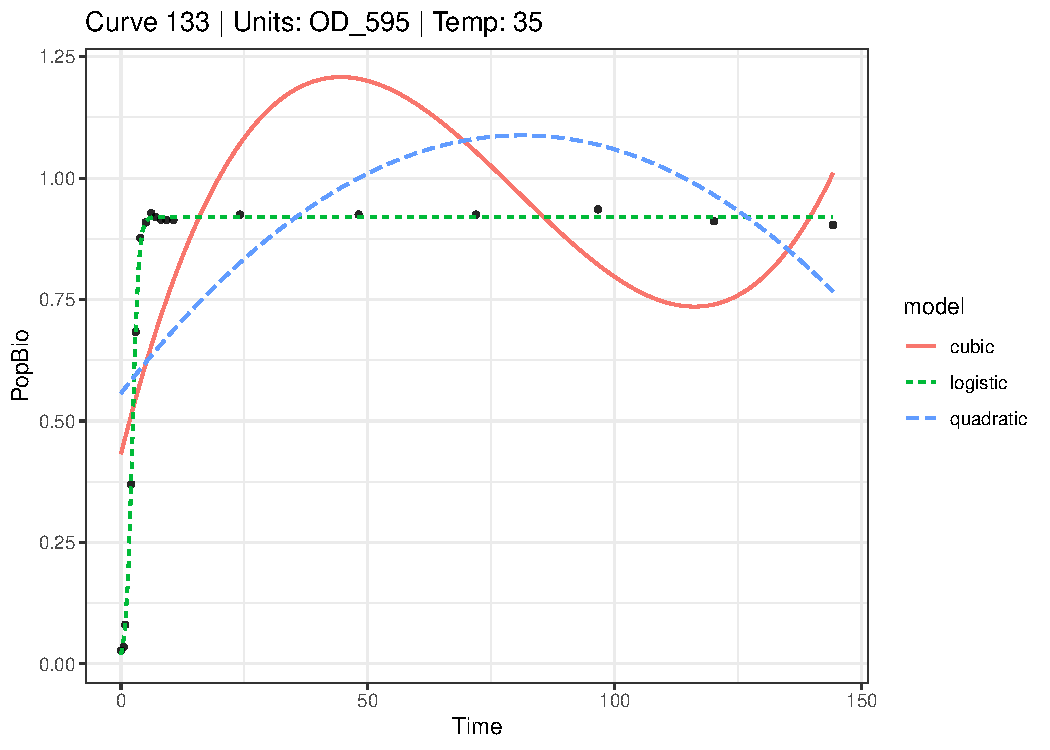
\includegraphics[width=\textwidth]{plots/curve_133.pdf}
    \caption{Curve 133: strong logistic win}
    \label{fig:curve133}
\end{subfigure}
\hfill
\begin{subfigure}[b]{0.48\textwidth}
    \centering
    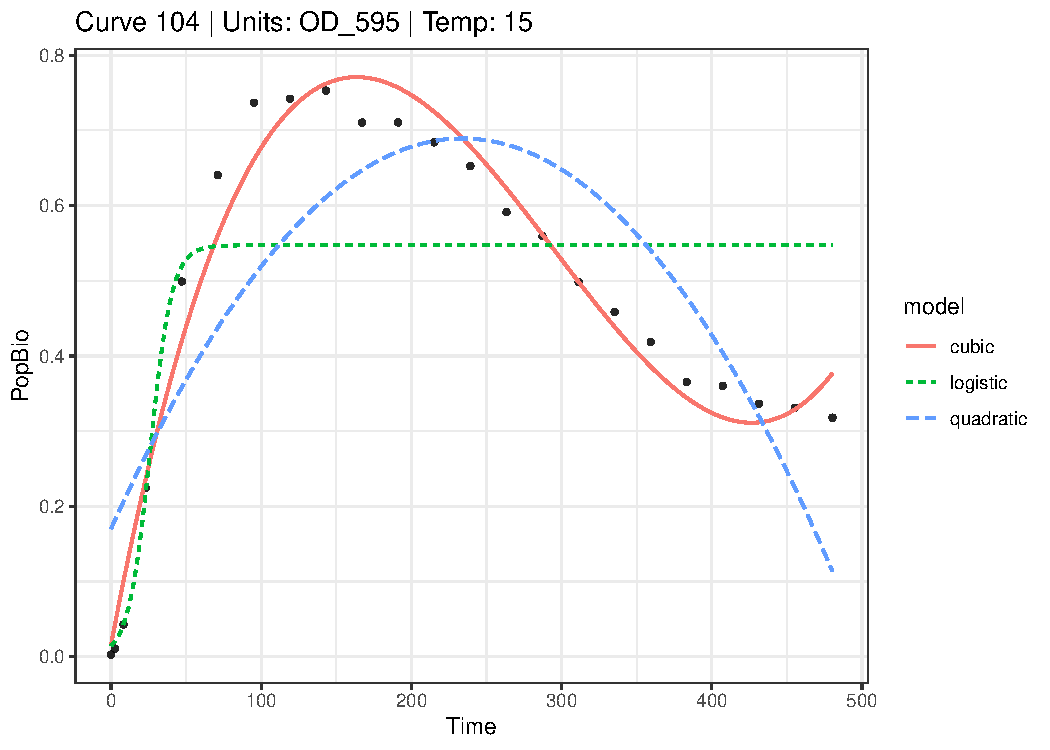
\includegraphics[width=\textwidth]{plots/curve_104.pdf}
    \caption{Curve 104: strong cubic win}
    \label{fig:curve104}
\end{subfigure}

\vspace{0.6em}

\begin{subfigure}[b]{0.48\textwidth}
    \centering
    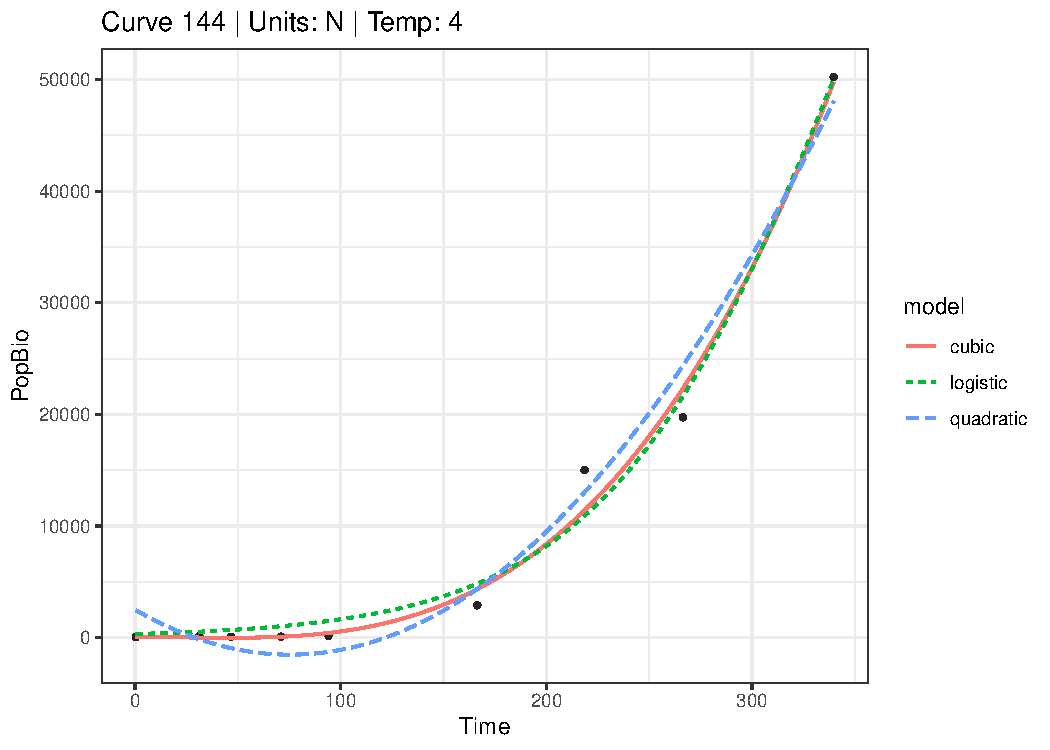
\includegraphics[width=\textwidth]{plots/curve_144.pdf}
    \caption{Curve 144: borderline logistic case}
    \label{fig:curve144}
\end{subfigure}
\hfill
\begin{subfigure}[b]{0.48\textwidth}
    \centering
    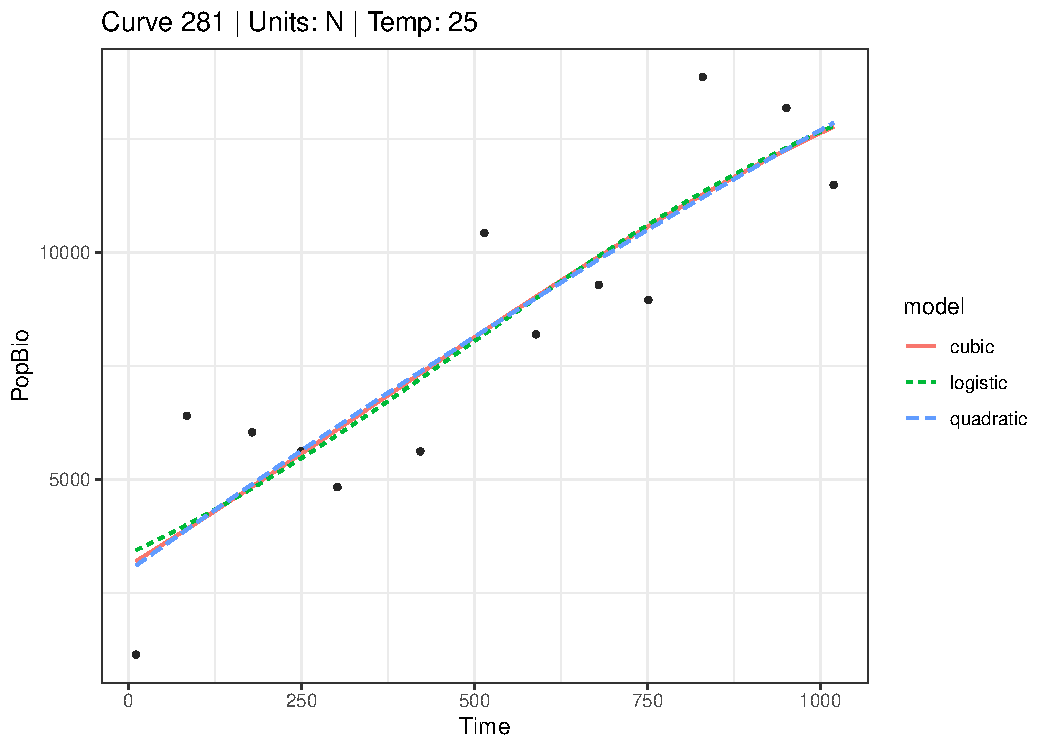
\includegraphics[width=\textwidth]{plots/curve_281.pdf}
    \caption{Curve 281: borderline quadratic case}
    \label{fig:curve281}
\end{subfigure}
\caption{Representative fitted curves selected to illustrate the main outcome patterns. Black points show the observed data for each microbial growth curve, and coloured lines show fitted values from the three candidate models. Panel (a) shows a clean sigmoidal trajectory strongly favoured by the logistic growth model. Panel (b) shows a curve with clear post-peak decline that was better captured by the cubic model. Panels (c) and (d) show borderline cases in which the best-supported model was only weakly separated from the alternatives.}
\label{fig:rep_curves}
\end{figure}